\documentclass[a4paper, 11pt, titlepage]{article}
\setlength{\oddsidemargin}{0in} \setlength{\evensidemargin}{0in}
\setlength{\textwidth}{6.2in}
\setlength{\topmargin}{-0.2in} \setlength{\textheight}{8.8in}

\usepackage{pdflscape}
\usepackage{graphicx}
\graphicspath{ {images/} }

\title{SE31520 Assignment 1 - Part 2: Forum for the CSA - version 1}
\author{Michal Wojciech Goly [mwg2]}
\date{30th November 2017}

\begin{document}

\maketitle
\tableofcontents
\newpage

\section{Introduction}
This document describes the architecture of the forum feature added to the CSA application
as part of the assignment submission for the SE31520 module at Aberystwyth University. The
following sections describe the design and implementation choices made during the development,
alongside testing performed and the implementation of the REST API. The report finishes with
the summary of the activities performed to achieve "flair" marks and sums up the work with
a critical evaluation.

\section{The CSA application}
I started the development by familiarising myself with the initial CSA architecture and
thinking about different ways I could add the forum functionality required. The Entity Relationship
Diagram below depicts the overall database schema of the final system, but my initial low fidelity
sketch included only the \texttt{Topics}, \texttt{Posts} and \texttt{Users} tables.

\subsection{Entity Relationship Diagram}
\begin{center}
  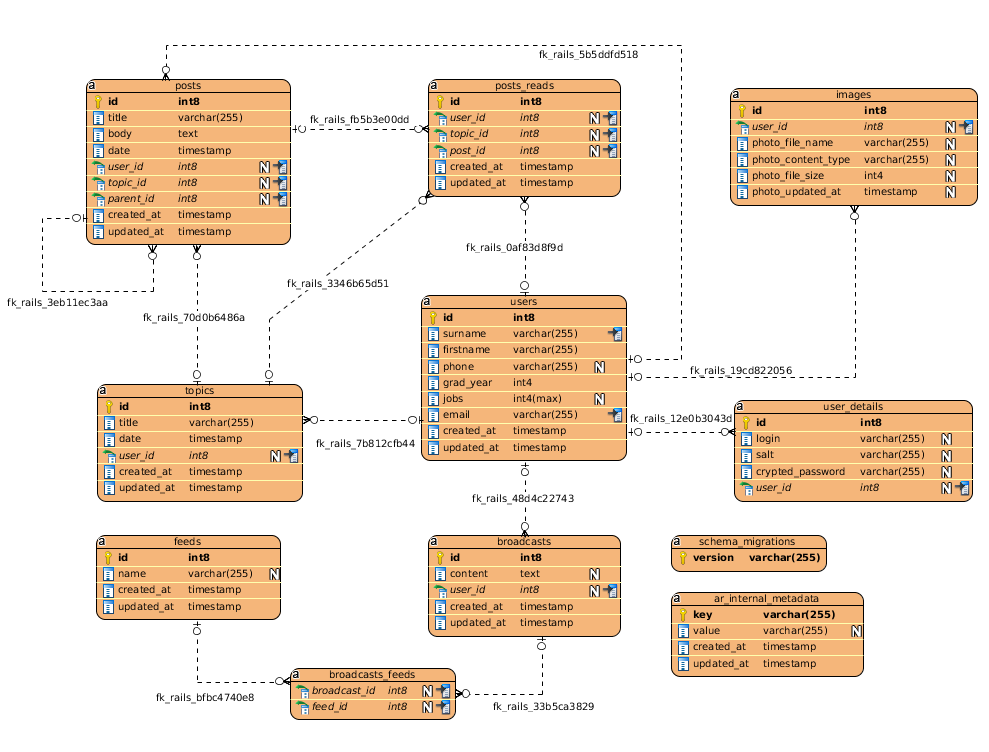
\includegraphics[scale=0.5]{schema}
\end{center}

\subsection{The forum feature}
Once the initial planning phase has finished, I have created a GitHub repository for the project,
created work items, Dockerised the project, integrated it with Circle CI and continuously deployed the \texttt{master}
branch to Heroku (I have covered the details in the \textit{Flair} section of this document).

Having cleaned up the CSS and fixed the broken migrations provided (timestamps were in a wrong order),
I have scaffolded the \texttt{Topic} migration, model, controller and views. I then added a
\textit{Forum} tab in the navbar and scaffolded the \texttt{Post} in a similar fashion. I wanted
to generate as much as possible early on and then remove "dead code" once the forum functionality
was implemented. The scaffolded code was not ideal and I had to manually define the \texttt{belongs\_to}
and \texttt{has\_many} relations between the models. I also used self joins to make sure each \texttt{Post}
could have a parent to represent posts' replies.

New topics can be created by calling the \texttt{/topics/new} route which will trigger the \texttt{TopicsController\#new}
action. Now, instead of creating a new \texttt{Topic} model and passing it to the view, I decided to create
a \texttt{Post}, pass it to the view and use partial rendering to reuse the \texttt{/views/posts/\_form.html.erb}
view for both \texttt{Topic} creation and \texttt{Post} replies later on. Logically, \texttt{Topic} cannot exist on its own
therefore such approach seemed optimal to minimise the amount of code written.

Implementation of the post replies and the associated indenting was argubly the most interesting
part of the assignment. The \texttt{/views/topics/show.html.erb} view uses material design cards to
render each post. The indentation was achieved using the Materialize CSS\cite{1} grid system.
The \texttt{Topic\#post\_wrappers} method iterates over the posts of a topic, recursively sorts
them and calculates the offsets based on the amount of parents above a specific node. These wrappers
are then returned as a simple array back to the view and rendered appropriately.

Finally, I have added the anonymous posting by treating \texttt{nil} valued \texttt{User} of a \texttt{Topic} or \texttt{Post}
appropriately, the total count of posts for each \texttt{Topic} and the unread posts counter. This required the creation of a new
table in the database with the associated model \texttt{PostsRead}. I took the simple approach of storing 3 foreign keys
for a \texttt{User}, \texttt{Topic} and \texttt{Post}. This allowed me to add new records to this table each time user
accessed the \texttt{/views/topics/show.html.erb} view and render the counter in the topics list.

\subsection{Controllers Diagram}
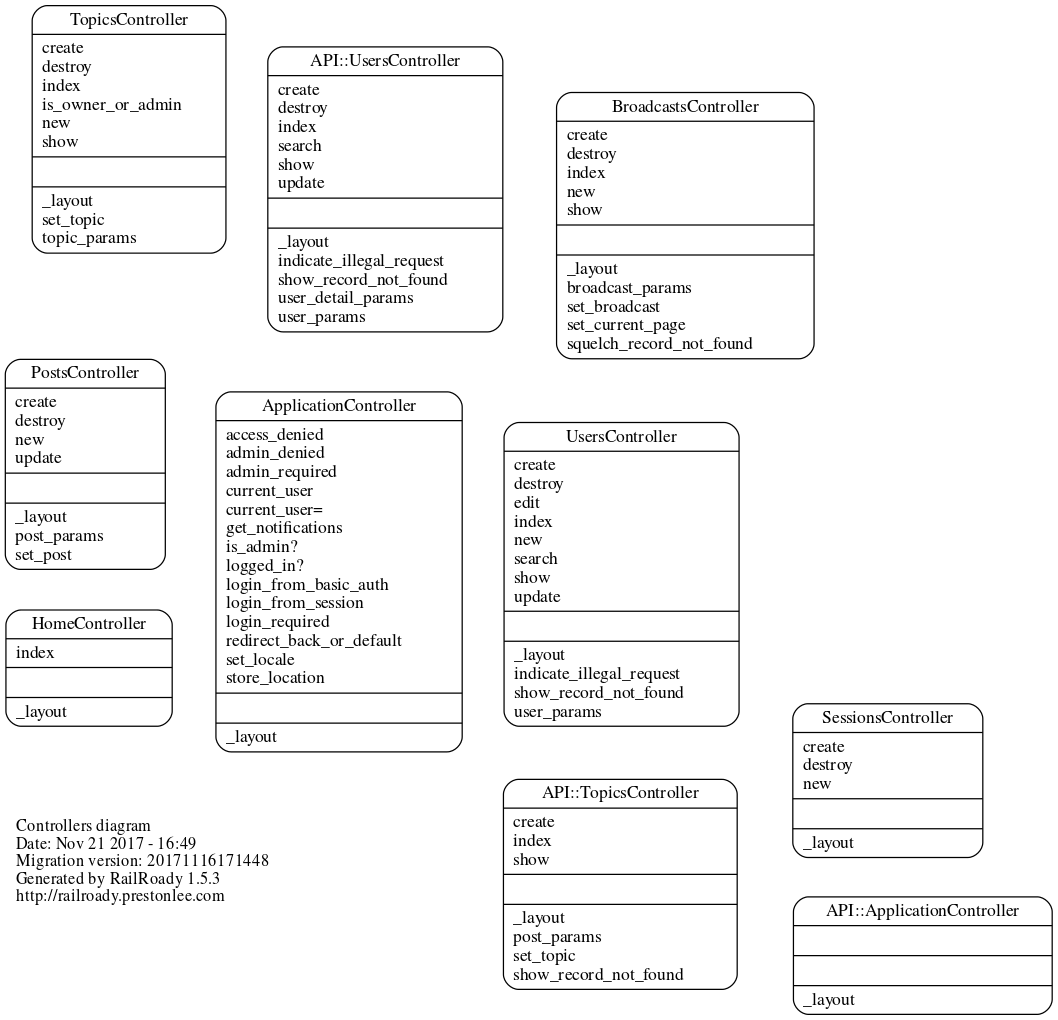
\includegraphics[scale=0.5]{controllers}
% rotate the page
\begin{landscape}

  \subsection{Models Diagram}
  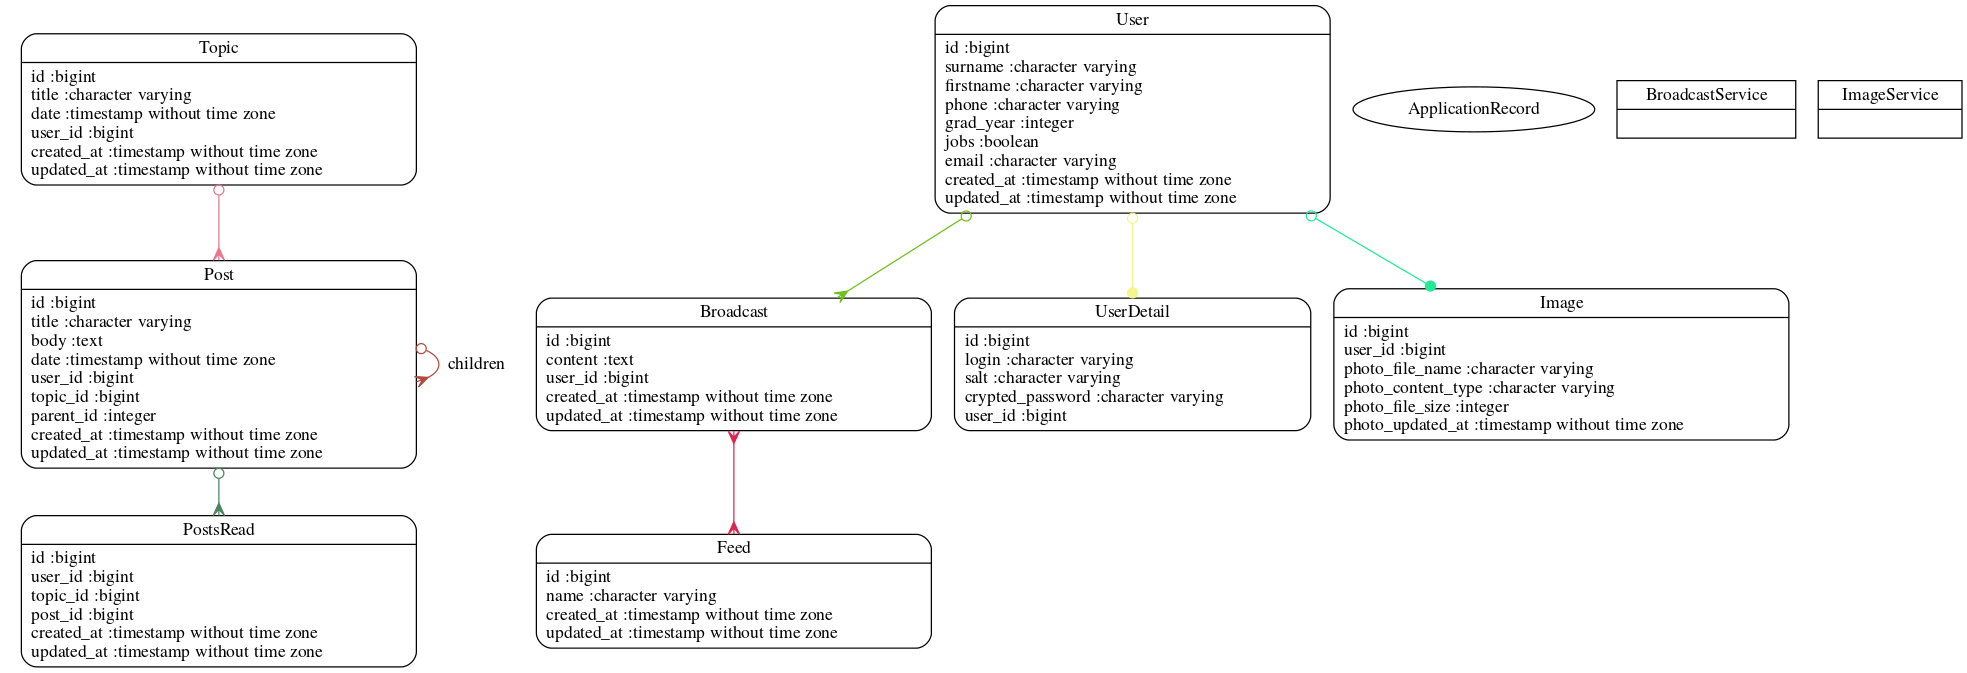
\includegraphics[scale=0.5]{models}
\end{landscape}

\subsection{Redesign for the REST API}


\section{The REST client}

\section{Cucumber testing}

\section{Flair}
\subsection{The overall look and feel}
Materialize CSS

\subsection{Docker}
Docker and Docker Compose of test and dev environments

\subsection{Build and extra testing}
Circle CI, running integration, cucumber tests, deployment of master to a production environment

\subsection{Heroku}
link to the deployment env

\subsection{Feature branches and Kanban}
the development process, pull requests, screenshot of the kanban board

\section{Critical evaluation}
- Could have added controller tests, but did not know how to mock sessions in rails 5
- Improve the look and feel of the rest of the app

\begin{thebibliography}{1}

\bibitem{1} \emph{Materialize CSS}, materializecss.com [Online],
Available: http://materializecss.com/grid.html, [Accessed: Nov. 22, 2017].

\end{thebibliography}

\end{document}
